% SELECT COUNT(*) FROM Wallet WHERE inferred=0; (before clustering)
\newcommand{\startingNumberAllWallets}{10477}

% SELECT COUNT(*) FROM Wallet WHERE Status != -1 and inferred=0; (before
% clustering)
\newcommand{\startingNumberWalletsNotService}{6603}

% SELECT COUNT(*) FROM Wallet WHERE Status = 1; (before clustering)
\newcommand{\startingNumberWalletsAtLeastOneTransaction}{1741}

% SELECT COUNT(*) FROM Wallet WHERE 1; (after clustering)
\newcommand{\clusteringNumberAllWallets}{16910}

% SELECT COUNT(*) FROM Wallet WHERE Status != -1; (after clustering)
\newcommand{\clusteringNumberWalletsNotService}{13036}

% SELECT COUNT(*) FROM Wallet WHERE Status != -1 AND Currency='BTC' and
% inferred=0;
% (before clustering)
\newcommand{\startingBTC}{1953}

% SELECT COUNT(*) FROM Wallet WHERE Status != -1 AND Currency='DOGE' and
% inferred=0;
% (before clustering)
\newcommand{\startingDOGE}{654}

% SELECT COUNT(*) FROM Wallet WHERE Status != -1 AND Currency='LTC' and
% inferred=0;
% (before clustering)
\newcommand{\startingLTC}{813}

% SELECT COUNT(*) FROM Wallet WHERE Status != -1 AND Currency='XMR' and
% inferred=0 ;
\newcommand{\startingXMR}{228}

% SELECT COUNT(*) FROM Wallet WHERE Status != -1 AND Currency='ETH' and
% inferred=0;
\newcommand{\startingETH}{2953}

% SELECT COUNT(*) FROM Account WHERE 1;
\newcommand{\accountNumber}{3444}

% SELECT (x*1.0)/((y-1)*1.0) FROM
% (
%     SELECT COUNT(*) AS x
%     FROM Wallet
%     WHERE Wallet.Status != -1
% ),
% (
%     SELECT COUNT(*) AS y
%     FROM Account
% )
\newcommand{\avarageAccount}{$~$3.786}

%~ SELECT COUNT(*) FROM (SELECT DISTINCT * FROM AccountRelated)
\newcommand{\accountRelated}{275}

%~ SELECT count(*) FROM Account WHERE host = 'twitter.com'
\newcommand{\accountTwitter}{888}

%~ SELECT sum(x, y) FROM SELECT count(*) as x FROM Account WHERE host =
% 'github.com',
\newcommand{\accountGithub}{2215}

%~ SELECT count(*) as y FROM Account WHERE host LIKE 'bitcointalk.org'
\newcommand{\accountBitcointalk}{337}

%~ SELECT count(*) FROM Account WHERE host LIKE 'gitlab.com'
\newcommand{\accountGitlab}{2}

%~ SELECT count(*) FROM Account WHERE host LIKE 'bitbucket.org'
\newcommand{\accountBitbucket}{1}


\section{Results} \label{results}
After we implemented and tested \texttt{Nduja} we ran it. The first step of the
algorithm gave us \startingNumberAllWallets{} addresses,
\startingNumberWalletsNotService{} addresses that probably are not services,
but only \startingNumberWalletsAtLeastOneTransaction{} of them we were able to
attest that they had at least one transaction. We found out \startingBTC{}
Bitcoin addresses, \startingLTC{} Litecoin addresses, \startingDOGE{}
addresses, \startingETH{} addresses and finally \startingXMR{} Monero
addresses. This is depicted in~\autoref{fig:numberaccountcurrency}.


\begin{figure*}
\centering
\begin{subfigure}[t]{0.3\textwidth}
\centering
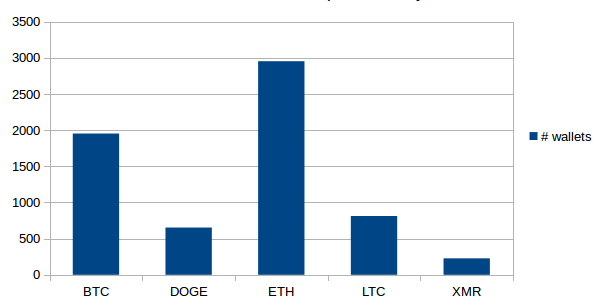
\includegraphics[width=.9\textwidth, height=3.5cm]{number_account_currency}
\caption{Number of wallets retrieved for each currency}
\label{fig:numberaccountcurrency}
\end{subfigure}
~
\begin{subfigure}[t]{0.3\textwidth}
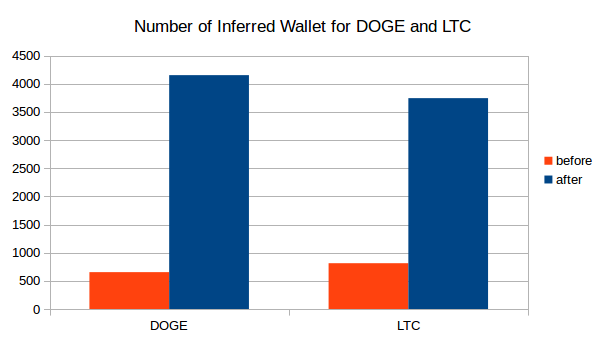
\includegraphics[width=.9\textwidth, height=3.5cm]{number_inferred_DOGE_LTC}
\caption{Comparison between the number of wallets before and after clustering
for DOGE and LTC}
\label{fig:dogeltcclustered}
\end{subfigure}
~
\begin{subfigure}[t]{0.3\textwidth}
\centering
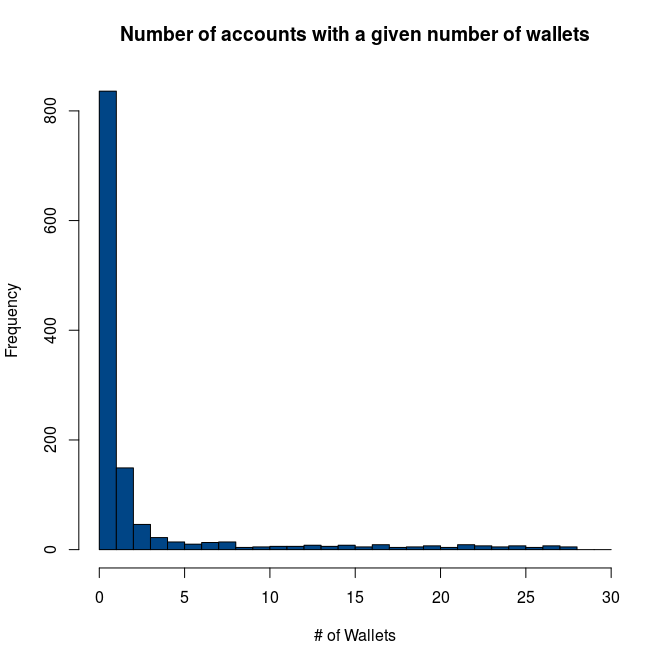
\includegraphics[width=.9\textwidth, height=3.5cm]{numwall}
\caption{Distribution of the number of wallets per account}
\label{fig:numwall}
\end{subfigure}
\caption{Results of our study}
\end{figure*}
As we expected the currency on which, potentially, we could retrieve more data
is still Bitcoin. The number of Monero wallets found is \startingXMR{} and it
could be so low even because it is an altcoin not so used and it was born in
order to preserve users privacy, so people could be more aware to advertise it.
From those wallets \accountGithub{} came by searching Github, \accountTwitter{}
from Twitter. Exploiting Github search we found other \accountBitcointalk{}
accounts that are related to \url{bitcointalk.org} forum, because one of the
repository listed them. Searchcode did not give us a useful improvement
because we were able only to retrieve other 3 addresses (\accountGitlab{} from
Gitlab and \accountBitbucket{} from Bitbucket) that were not already present in
the Github's wallets.
After that we ran the clustering procedure \emph{only} on Litecoin and Dogecoin
addresses. We excluded Bitcoin wallets due to time constraints.
For further details we
refer to~\autoref{sec:issues}. Ethereum and Monero were not considered
because the first does not allow multiple-input transactions, so it is not
possible to cluster wallets as for the other, instead the latter has private
transactions, so it is not possible to analyze its transaction history.
After the clustering, we increase the number of addresses discovered to
\clusteringNumberAllWallets{}, with \clusteringNumberWalletsNotService{}
wallets, without considering known services.
In~\autoref{fig:dogeltcclustered} is depicted the increase of the number of
wallets found.
Addresses are connected to \accountNumber{} accounts and on average we had
\avarageAccount{} addresses per person.
The distribution of the number of wallets per account is represented
in~\autoref{fig:numwall}. We considered only accounts with at most 28 related
wallets by setting a maximum limit on the number of
wallets to spare time.
Therefore if a wallet had more than 29 wallets we could not assert whether
the account had actually 29 addresses or more.
We were able to connect Facebook or Linkedin accounts to some of the wallets.
In particular the latter social network is the most interesting, because people
are more likely to share sensitive data on that because of its aim.
Finally, \accountRelated{} accounts in our database are strongly related with
at least another one: this means that one of their addresses are used together
as input in the same transaction. During the analysis of those relations we
found out that some of them are ``spurious'': the wallets seems to belong to
different people.
